\documentclass[
11pt, % The default document font size, options: 10pt, 11pt, 12pt
codirector, % Uncomment to add a codirector to the title page
]{charter} 




% El títulos de la memoria, se usa en la carátula y se puede usar el cualquier lugar del documento con el comando \ttitle
\titulo{Sistema de control para un robot tetrápodo} 

% Nombre del posgrado, se usa en la carátula y se puede usar el cualquier lugar del documento con el comando \degreename
%\posgrado{Carrera de Especialización en Sistemas Embebidos} 
%\posgrado{Carrera de Especialización en Internet de las Cosas} 
%\posgrado{Carrera de Especialización en Intelegencia Artificial}
\posgrado{Maestría en Sistemas Embebidos} 
%\posgrado{Maestría en Internet de las cosas}

% Tu nombre, se puede usar el cualquier lugar del documento con el comando \authorname
\autor{Ing. Pablo Daniel Folino} 

% El nombre del director y co-director, se puede usar el cualquier lugar del documento con el comando \supname y \cosupname y \pertesupname y \pertecosupname
\director{Ing. Juan Carlos Gómez}
\pertenenciaDirector{INTI,UTN.BA} 
% FIXME:NO IMPLEMENTADO EL CODIRECTOR ni su pertenencia
\codirector{} % para que aparezca en la portada se debe descomentar la opción codirector en el documentclass
\pertenenciaCoDirector{}

% Nombre del cliente, quien va a aprobar los resultados del proyecto, se puede usar con el comando \clientename y \empclientename
\cliente{Ing. Claudio Verrastro}
\empresaCliente{UTN-FRBA-GIAR}

% Nombre y pertenencia de los jurados, se pueden usar el cualquier lugar del documento con el comando \jurunoname, \jurdosname y \jurtresname y \perteunoname, \pertedosname y \pertetresname.
\juradoUno{Nombre y Apellido (1)}
\pertenenciaJurUno{pertenencia (1)} 
\juradoDos{Nombre y Apellido (2)}
\pertenenciaJurDos{pertenencia (2)}
\juradoTres{Nombre y Apellido (3)}
\pertenenciaJurTres{pertenencia (3)}
 
\fechaINICIO{21 de junio de 2021}		%Fecha de inicio de la cursada de GdP \fechaInicioName
\fechaFINALPlan{20 de agosto de 2021} 	%Fecha de final de cursada de GdP
\fechaFINALTrabajo{22 de agosto de 2022}	%Fecha de defensa pública del trabajo final


\begin{document}

\maketitle
\thispagestyle{empty}
\pagebreak


\thispagestyle{empty}
{\setlength{\parskip}{0pt}
\tableofcontents{}
}
\pagebreak


\section*{Registros de cambios}
\label{sec:registro}


\begin{table}[ht]
\label{tab:registro}
\centering
\begin{tabularx}{\linewidth}{@{}|c|X|c|@{}}
\hline
\rowcolor[HTML]{C0C0C0} 
Revisión & \multicolumn{1}{c|}{\cellcolor[HTML]{C0C0C0}Detalles de los cambios realizados} & Fecha      \\ \hline
0      & Creación del documento                                 &\fechaInicioName \\ \hline
1      & Se completa hasta el punto 2 inclusive                 & 25 de junio de 2021 \\ \hline
2      & Se completa hasta el punto 7 inclusive					& 02 de julio de 2021 \\ \hline
3	   & Se completa hasta el punto 10 inclusive 				& 06 de julio de 2021 \\ \hline
%		  En distintas líneas \newline
%		  Así                                                    & dd/mm/aaaa \\ \hline
%3      & Se completa hasta el punto 11 inclusive                & dd/mm/aaaa \\ \hline
%4      & Se completa el plan	                                 & dd/mm/aaaa \\ \hline
\end{tabularx}
\end{table}

\pagebreak

\section*{Acta de constitución del proyecto}
\label{sec:acta}

\begin{flushright}
Buenos Aires, \fechaInicioName
\end{flushright}

\vspace{2cm}

Por medio de la presente se acuerda con el Ing. \authorname\hspace{1px} que su Trabajo Final de la \degreename\hspace{1px} se titulará ``\ttitle'', consistirá esencialmente en la implementación de un prototipo de un sistema de control de movimientos para un robot tetrápodo de tres grados de libertad en cada extremo, y tendrá un presupuesto preliminar estimado de 600 hs de trabajo y \textcolor{red}{\$XXX}, con fecha de inicio \fechaInicioName\hspace{1px} y fecha de presentación pública \fechaFinalName.

Se adjunta a esta acta la planificación inicial.

\vfill

% Esta parte se construye sola con la información que hayan cargado en el preámbulo del documento y no debe modificarla
\begin{table}[ht]
\centering
\begin{tabular}{ccc}
\begin{tabular}[c]{@{}c@{}}Ariel Lutenberg \\ Director posgrado FIUBA\end{tabular} & \hspace{2cm} & \begin{tabular}[c]{@{}c@{}}\clientename \\ \empclientename \end{tabular} \vspace{2.5cm} \\ 
\multicolumn{3}{c}{\begin{tabular}[c]{@{}c@{}} \supname \\ Director del Trabajo Final\end{tabular}} \vspace{2.5cm} \\
%\begin{tabular}[c]{@{}c@{}}\jurunoname \\ Jurado del Trabajo Final\end{tabular}     &  & \begin{tabular}[c]{@{}c@{}}\jurdosname\\ Jurado del Trabajo Final\end{tabular}  \vspace{2.5cm}  \\
%\multicolumn{3}{c}{\begin{tabular}[c]{@{}c@{}} \jurtresname\\ Jurado del Trabajo Final\end{tabular}} \vspace{.5cm}                                                                     
\end{tabular}
\end{table}




\section{1. Descripción técnica-conceptual del proyecto a realizar}
\label{sec:descripcion}


%\begin{consigna}{red} % El bloque "consigna" se usa para poner texto en rojo y dar una pequeña ayuda sobre cómo completar la sección

%El objetivo es que el lector en una o dos páginas entienda de qué se trata el proyecto y cuáles son sus desafíos, su motivación y su importancia.

%Se debe destacar claramente cuál es el valor que agrega el proyecto a realizar. ``El presente proyecto se destaca especialmente por incorporar tal cosa... Esto lo diferencia de otros sistemas similares en que ...''

%Puede ser útil incluir en esta sección la respuesta a alguna de estas preguntas:

%\begin{itemize}
%	\item ¿Cómo se vincula este proyecto con la misión de la organización?
%	\item ¿Cómo se inserta este proyecto en el modelo de negocio de la organización?
%	\item ¿Ayuda a la explicación si se incluye un lienzo Canvas del Modelo de Negocio?
%	\item ¿En qué estado del ciclo de vida está el producto que se desea reemplazar o mejorar?
%	\item ¿Cuáles son las necesidades que debe satisfacer?
%	\item ¿Por dónde pasa la innovación?
%\end{itemize}

%La descripción técnica-conceptual \textbf{debe incluir al menos un diagrama en bloques %del sistema} y una frase como la siguiente: ``En la Figura \ref{fig:diagBloques} se %presenta el diagrama en bloques del sistema. Se observa que...''. Luego recién más %abajo de haber puesto esta frase, se pone la figura. La regla es que las figuras nunca %pueden ir antes de ser mencionadas en el texto, porque sino el lector no entiende por %qué de pronto aparece una figura.

%\vspace{25px}



%\begin{figure}[htpb]
%\centering 
%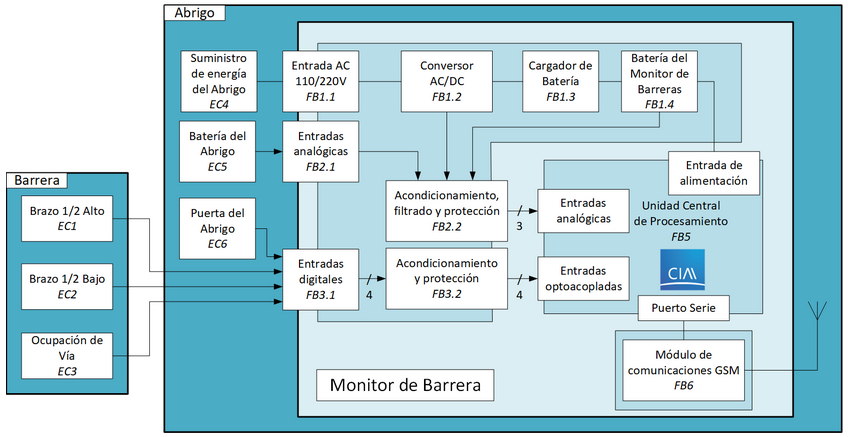
\includegraphics[width=.5\textwidth]{./Figuras/diagBloques.png}
%\caption{Diagrama en bloques del sistema}
%\label{fig:diagBloques}
%\end{figure}

%\vspace{25px}

%El tamaño de la tipografía en TODAS las figuras debe ser adecuado para que NO pase lo que ocurre acá, %donde el lector debe esforzarse para poder leer el texto. Los colores usados en el diagrama deben ser %adecuados, tal que ayuden a comprender mejor el diagrama, preferentemente en la gama de colores pastel.
%\end{consigna}


El objetivo es diseñar el hardware y firmware para controlar los movimientos de un robot tetrápodo de tres grados de libertad por cada extremo. El cerebro del sistema será una placa EDU-CIAA-NPX, que recibirá la información de los distintos sensores y controlará los actuadores. La placa recibirá información de comunicación por un módulo WIFI (del tipo ESP8266). 

En las articulaciones se utilizaran servomtores controlados por modulación de ancho de pulso(PWM-\textit{Pulse-width modulation}). 

El sistema (hardware-software) tiene que ser robusto para que permita realizar las distintas pruebas a las que se va a someter.

Uno de los principales problemas de los robots caminantes es su estabilidad, para ello se utilizara un módulo acelerómetro. Otro de los problemas es el consumo de los servomotores, por lo qué el sistema medirá la corriente de cada articulación.   

La generación y control de la locomoción en robots caminantes requiere de un esfuerzo computacional alto, tanto en el diseño como en la implementación. Es necesario coordinar los movimientos y trayectorias de todas las articulaciones de las extremidades del robot; lo cual resulta especialmente complicado cuando el número de extremidades aumenta, para ello se aplicarán algoritmos de Aprendizaje por Refuerzo (AR).

Antes de realizar la construcción física del prototipo se procederá a la simulación en un equipo informático, para tratar de evitar posibles problemas tanto en la construcción, como en el algoritmo de control empleado. 
El robot estará diseñado para moverse en espacios interiores (\textit{indoor}), en condiciones de temperaturas estándares entre 5 $^\circ$C y 40 $^\circ$C, y humedad relativa normales(entre 40 \% y 70 \% ).
También se minimizará la cantidad de piezas par que el sistema sea de bajo costo.  

El formato del robot será aproximadamente como lo muestra la Figura \ref{fig:robotTetrapodo}.
\begin{figure}[htpb]
\centering 
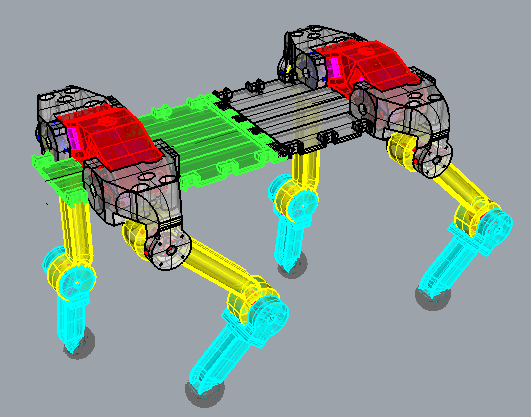
\includegraphics[width=.6\textwidth]{./Figuras/tetratopo.png}
\caption{Formato del robot propuesto.}
\label{fig:robotTetrapodo}
\end{figure}

En la Figura \ref{fig:robotDiagrama} se observan las relaciones entre los distintos componentes del sistema.

\begin{figure}[htpb]
\centering 
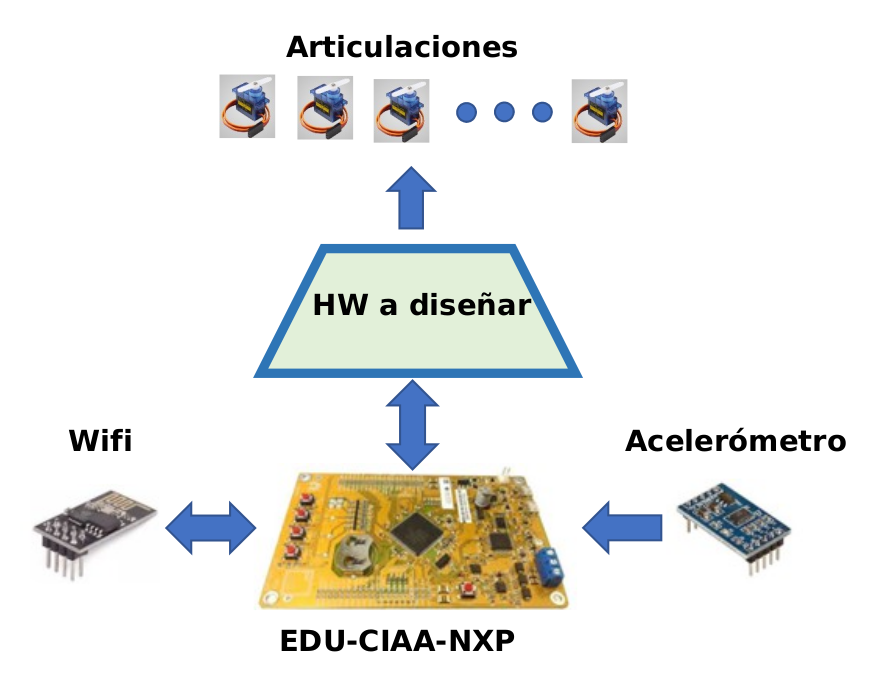
\includegraphics[width=.8\textwidth]{./Figuras/tetra.png}
\caption{Módulos de hardware del robot propuesto.}
\label{fig:robotDiagrama}
\end{figure}


\section{2. Identificación y análisis de los interesados}
\label{sec:interesados}

En esta plataforma se aplicarán algoritmos de Aprendizaje por Refuerzo (AR), se utilizara para formar recursos humanos dentro del Grupo de Inteligencia Artificial y Robótica (GIAR). Una vez afianzada la técnica, se realizará la transferencia de lo aprendido a los distintos clientes que posee el grupo de investigación, como materias afines de las distintas carreras de grado de la Universidad Tecnológica Nacional-Facultad Regional Buenos Aires.

\begin{table}[ht]
%\caption{Identificación de los interesados}
%\label{tab:interesados}
\begin{tabularx}{\linewidth}{@{}|l|X|X|l|@{}}
\hline
\rowcolor[HTML]{CCFFFF} 
Rol           & Nombre y Apellido & Organización 	& Puesto 	\\ \hline
%Auspiciante   & -  				& -					& -	   		\\ \hline
Cliente       & \clientename    &\empclientename	& -   		\\ \hline
Impulsor      & Lic. Patricia CIBEIRAT    		&\empclientename 	& Secretario de SeCyT    		\\ \hline
Responsable   & \authorname     & FIUBA        		& Alumno 	\\ \hline
Colaboradores & Miembros del GIAR   & UTN-FRBA     		& -       	\\ \hline
Orientador    & \supname	    & \pertesupname 	& Director	trabajo final \\ \hline
%Equipo        & -          		& -             	& -        	\\ \hline
Opositores    & Otros Grupos Invest.    & UTN-FRBA             	& -        	\\ \hline
Usuario final & Alumnos de materia -IA     &\empclientename	& -        	\\ \hline
\end{tabularx}
\end{table}

%El Director suele ser uno de los Orientadores.
%No dejar celdas vacías; si no hay nada que poner en una celda colocar un signo ``-''.
%No dejar filas vacías; si no hay nada que poner en una fila entonces eliminarla.

%Sería deseable listar a continuación de la tabla las principales características de cada interesado.
 
%Por ejemplo:
%\begin{itemize}
%\item Auspiciante: es riguroso y exigente con la rendición de gastos. Tener mucho cuidado con esto.
%\item Equipo: Juan Perez, suele pedir licencia porque tiene un familiar con una enfermedad. Planificar considerando esto.
%\item Orientador: María Gómez, nos va a poder ayudar mucho con la gestión de impuestos.
%\end{itemize}

%\end{consigna}

\begin{itemize}
\item Orientador: Ing. Juan Carlos Gómez, posee mucha experiencia en el tema debido a su trabajo, y formación  profesional, pero no posee mucho tiempo.
\item Cliente: posee muchas restricciones con respecto a los costos.
\end{itemize}


\section{3. Propósito del proyecto}
\label{sec:proposito}

El propósito del proyecto es diseñar el hardware y el firmware de un controlador de movimientos para un robot tetrápodo de tres grados de libertad en cada extremo, y aplicar los conocimientos en materias de inteligencia artificial dictadas en la UTN-FRBA.


\section{4. Alcance del proyecto}
\label{sec:alcance}

El objetivo del proyecto comprende:

\begin{itemize}
\item Diseñar y armar el prototipo del hardware del robot tetrápodo.
\item Diseñar e implementar en la placa EDU-CIAA-NXP el software embebido de A.R.
\item Diseñar comandos para cambiar el modo de funcionaniento desde línea de comandos, desde una PC. 
\item Realizar el proyecto dentro del tiempo destinado al mismo.
\end{itemize}

El proyecto no incluye:

\begin{itemize}
\item Realizar pruebas de estructuras de hardware, para saber la vida útil del sistema.
\item Diseñar una interface gráfica amigable para cambiar los distintos modos de funcionamiento.
\item Diseñar y/o armar el cargador de baterías.
\item El diseño del módulo de alimentación se lo dejará para un estado posterior a este proyecto, como así también las pruebas de autonomía.El objetivo del proyecto comprende:

\begin{itemize}
\item Diseñar y armar el prototipo del hardware del robot, tipo triciclo.
\item Diseñar e implementar en la placa EDU-CIAA-NXP el software embebido de A.R.
\item Diseñar comandos para cambiar el modo de funcionaniento desde línea de comandos, desde una PC. 
\item Realizar el proyecto dentro del tiempo destinado al mismo.
\end{itemize}

El proyecto no incluye:

\begin{itemize}
\item Realizar pruebas de estructuras de hardware, para saber la vida útil del sistema.
\item Diseñar una interface gráfica amigable para cambiar los distintos modos de funcionamiento.
\item Diseñar y/o armar el cargador de baterías.
\item Carcasa, ni gabinete para el robot.
\end{itemize}
\end{itemize}


\section{5. Supuestos del proyecto}
\label{sec:supuestos}

Se supone para el siguiente proyecto que:
\begin{itemize}
\item se posee el presupuesto para comprar todo lo relacionado con el hardware necesario para construir el robot. 
\item se contará con acceso a todo el equipamiento para la construcción y testeo de los distintos elementos electrónicos.
\item la complejidad de la programación se restringirá en función de las horas de trabajo propuestas para hacer este proyecto.
\item se podrá conseguir los distintos elementos electrónicos en este contexto de pandemia.
\end{itemize}

\section{6. Requerimientos}
\label{sec:requerimientos}

\begin{enumerate}
\item Requerimientos de funcionamiento general
	\begin{enumerate}
	\item El robot debe alimentarse mediante un sistema que le permita tener la posibilidad de desplazarse sin problemas.
	\item Se debe comunicar en forma inalámbrica y mediante el puerto USB de la placa EDU-CIAA-NXP. 
	\item El robot debe ser lo suficiente ligero para que los servomotores puedan mover las articulaciones .
	\end{enumerate}
\item Grupo de requerimientos asociados con el hardware
	\begin{enumerate}
	\item El hardware debe ser fácilmente replicable utilizando una impresora 3D.
	\item Debe poseer la menor cantidad de piezas posibles, no mayor a cuarenta. 
	\item El cuerpo del robot debe albergar todo el hardware (motores, placa EDU-CIAA, drivers de motores, , etc.) necesario para el funcionamiento normal.
	\item Debe poseer un botón de parada de emergencia de fácil acceso, para interrumpir el funcionamiento del robot en caso de urgencia.
	\end{enumerate}
\item Grupo de requerimientos asociados con el software
	\begin{enumerate}
	\item Se programará usando Lenguaje C, utilizando el modelo de capas y las sAPI del proyecto CIAA.
	\item La herramienta de programación en Lenguaje C deberá poseer un modo DEBUG.
	\item El uso de memoria no debe exceder a la placa EDU-CIAA-NXP.
	\end{enumerate}
\item Requerimientos no funcionales
	\begin{enumerate}
	\item La estructura del robot no debe tener bordes filosos ni punzantes, que puedan ocasionar lesiones. 
	\item La velocidad que desarrolla el robot debe ser inferior a 1 m/seg.
	\end{enumerate}

\vspace{2cm} 

\item Requerimientos documentación
	\begin{enumerate}
	\item Redactar el manual de uso. 
	\item Redactar un documento en donde se registre el código 
	fuente.
	\item Redactar un documento técnico que figuren los circuitos
	esquemáticos, y el armado de la plataforma.
	\end{enumerate}
\end{enumerate}

\section{7. Historias de usuarios (\textit{Product backlog})}
\label{sec:backlog}

Criterio: a mayor valor de prioridad, la historia de usuario es más importante. Para el grado de ponderación se toma el criterio horas-hombre (valor de esfuerzo) que supone la implementación de la historia de usuario.

\begin{itemize}
\item Historia de usuario 1: Como docente quiero que el robot se pueda conectar a una red local, para poder controlarlo desde una posición remota.
	\begin{itemize}
	\item Prioridad : 1
	\item Ponderación : 5
	\end{itemize}
\item Historia de usuario 2: Como alumno quiero poder cambiar los distintos algoritmos de control, para poder sintonizar los movimientos de la plataforma móvil. 
	\begin{itemize}
	\item Prioridad : 2
	\item Ponderación : 5
	\end{itemize}	
\item Historia de usuario 3:  Como alumno quiero tener una aplicación  gráfica en un dispositivo móvil, para poder manejar los movimientos del robot mediante \textit{wifi} o el puerto USB. 
	\begin{itemize}
	\item Prioridad : 3
	\item Ponderación : 7
	\end{itemize}
\item Historia de usuario 4: Como ayudante de laboratorio encargado del robot quiero que se pueda reparar rápidamente, para no perder tiempo. 
	\begin{itemize}
	\item Prioridad : 4
	\item Ponderación : 3
	\end{itemize}	
\item Historia de usuario 5: Como docente quiero tener la posibilidad de contar con una fuente de energía a baterías para poder usar el robot en cualquier ambiente.
	\begin{itemize}
	\item Prioridad : 5
	\item Ponderación : 1
	\end{itemize}		
\end{itemize}

\vspace{4cm} 

\section{8. Entregables principales del proyecto}
\label{sec:entregables}

Al final del proyecto se entregará: 
\begin{itemize}
\item Prototipo del robot.
\item Manual de uso.
\item Diagrama esquemático.
\item Código fuente.
\item Diagrama de instalación.
\item Informe final..
\end{itemize}


\section{9. Desglose del trabajo en tareas}
\label{sec:wbs}

\begin{enumerate}
\item Planificación de tareas. (40 hs)
	\begin{enumerate}
	\item Generación del documento de planificación del proyecto. (30 hs)
	\item Aprobación y revisión del documento de planificación del proyecto. (10 hs)
	\end{enumerate}
\item Investigación preliminar del hardware a utilizar. (38 hs)
	\begin{enumerate}
	\item Fabricación del robot. (20 hs)
	\item Placas electrónicas(placa principal, microcontrolador, drivers, etc). (10 hs)
	\item Características de los motores.  (4 hs)
	\item Características de las fuente de alimentación. (4 hs)
	\end{enumerate}
\item Selección y compra de los materiales del hardware. (8 hs)
	\begin{enumerate}
	\item Selección de los componentes. (5 hs)
	\item Compra y adquisición.(3 hs)
	\end{enumerate}
\item Armado y verificación de la estructura del robot. (43 hs)
	\begin{enumerate}
	\item Construcción de las piezas. (30 hs)
	\item Ensamblaje de piezas. (3 hs)
	\item Verificación de la estructura. (10 hs)
	\end{enumerate}
\item Armado y verificación de la electrónica del robot. (10 hs)
	\begin{enumerate}
	\item Armado de la placa adaptadora entre EDU-CIAA y los distintos módulos. (5 hs)
	\item Cableado del robot. (2 hs)
	\item Verificación de la electrónica. (3 hs)
	\end{enumerate}	

\vspace{4cm} 

\item Integración del hardware. (6 hs)	
\item Desarrollo del software (189hs)
	\begin{enumerate}
	\item Módulo PWM. (25 hs)
	\item Módulo WIFI y protocolo de comunicaciones. (44 hs)
	\item Módulo acelerómetro.  (25 hs)
	\item Módulo de aprendizaje por refuerzo. (40 hs)
	\item Módulo manual. (25 hs)
	\item Integración de los distintos módulos. (30 hs)
	\end{enumerate}	
\item Verificación del software(\textit{Testing}). (75 hs)
	\begin{enumerate}
	\item Diseño de pruebas  de ensayo de los distintos módulos. (25 hs)
	\item Diseño de las distintas pruebas de navegación. (30 hs)
	\item Comparación de las distintas estrategias de navegación. (20 hs)
	\end{enumerate}	
\item Validación del sistema completo. (40 hs)
	\begin{enumerate}
	\item Ensayos de verificación del cliente en forma parcial. (20 hs)
	\item Ensayos de validación final. (20 hs)
	\end{enumerate}	
\item Presentación del trabajo. (151 hs)
	\begin{enumerate}
	\item Redacción de informes de avance. (10 hs)
	\item Redacción de manual de uso. (20 hs)
	\item Elaboración de circuitos esquemáticos. (20 hs)
	\item Redacción de memoria del proyecto. (80 hs)
	\item Preparación de la presentación pública del trabajo final. (20 hs)
	\item Presentación pública del trabajo final. (1 h)
	\end{enumerate}					
\end{enumerate}
Cantidad total de horas: (600 hs)

\pagebreak

\section{10. Diagrama de Activity On Node}
\label{sec:AoN}

En la figura \ref{fig:AoN}, se observa el camino crítico en color rojo. La unidad de tiempo definida en cada tarea es en hora.
 
\begin{figure}[htpb]
\centering 
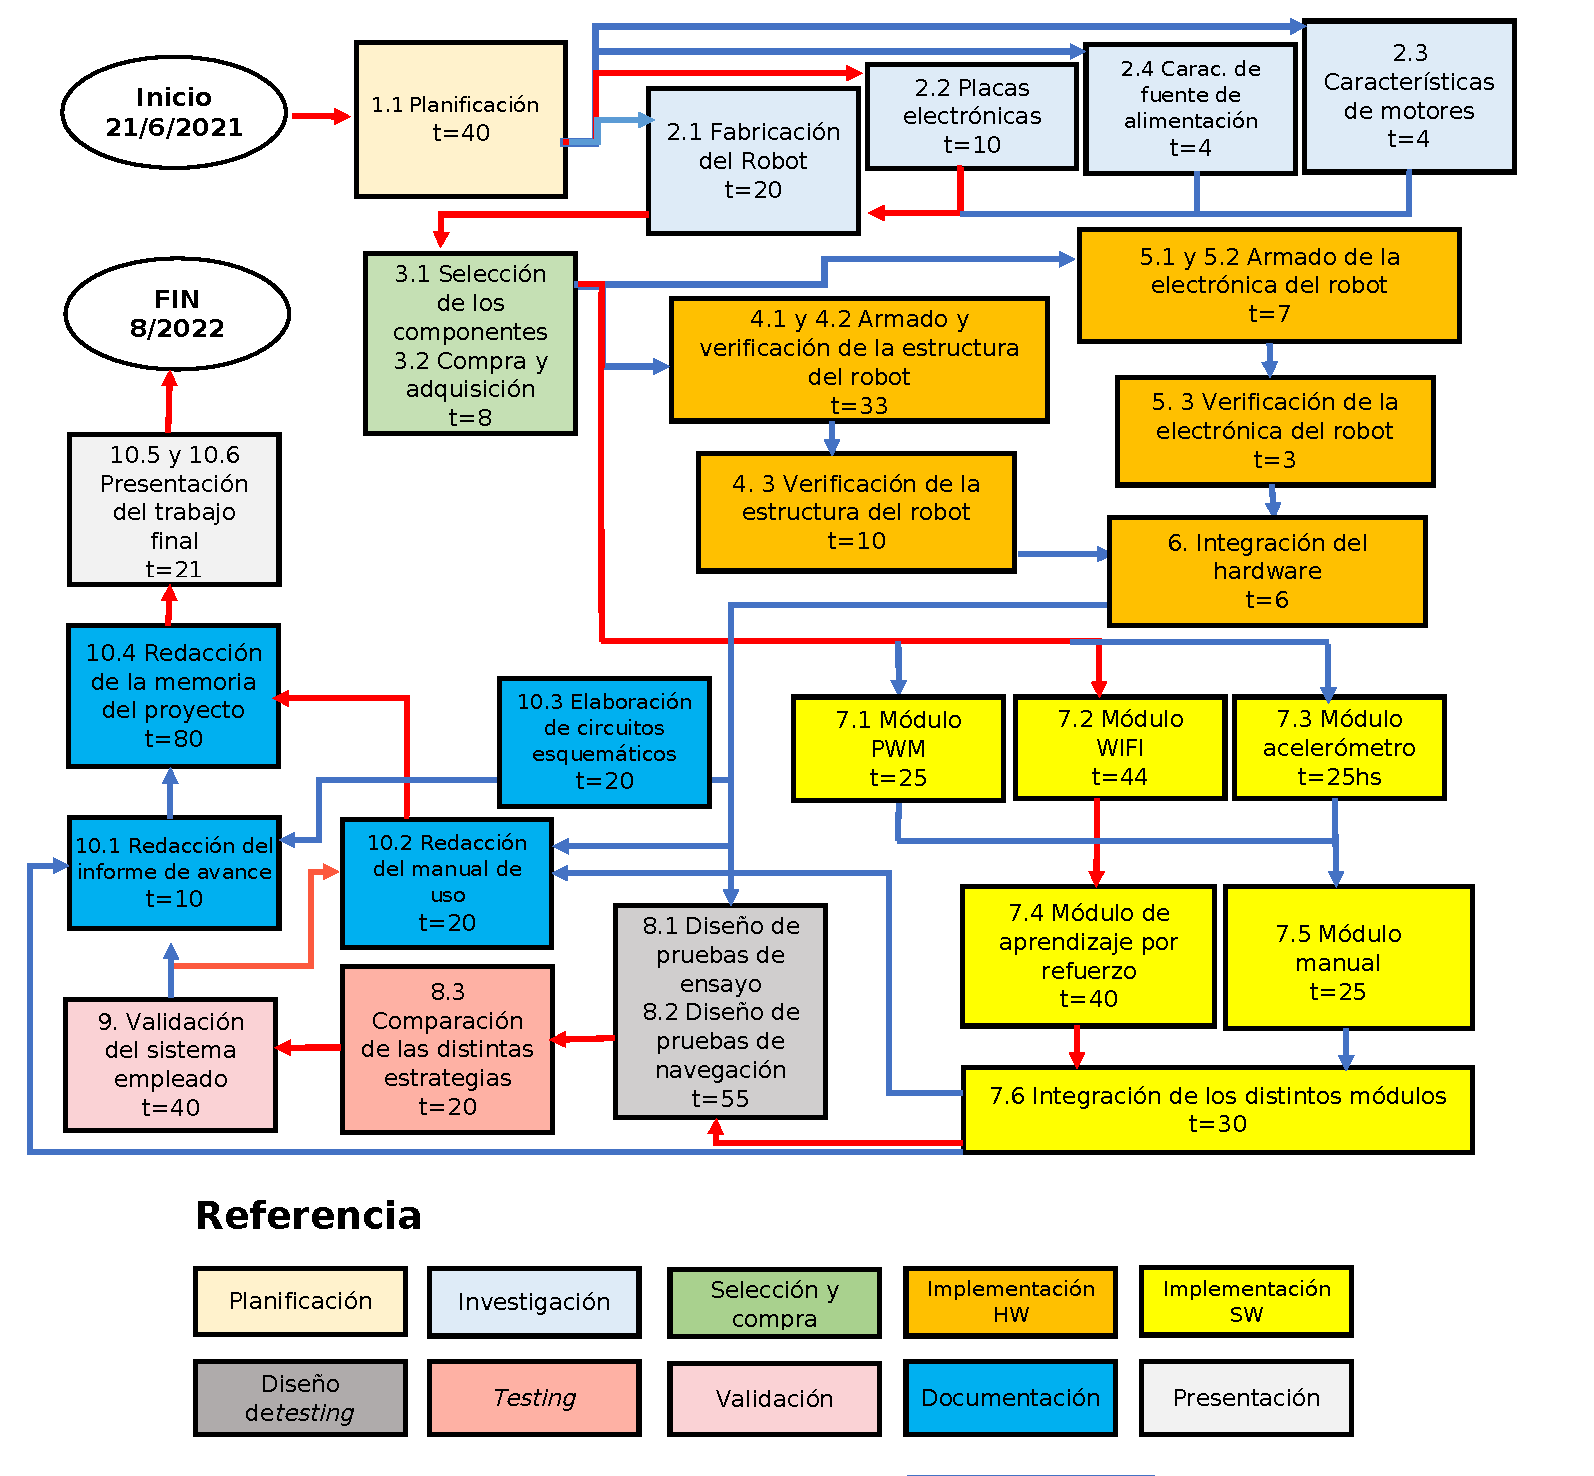
\includegraphics[width=\textwidth]{./Figuras/AoN.pdf}
\caption{Diagrama de \textit{Activity on Node}}
\label{fig:AoN}
\end{figure}


\section{11. Diagrama de Gantt}
\label{sec:gantt}

Los datos de la tabla 1 y de la figura 4 se obtuvieron de un software de gestión de proyectos teniendo en cuenta los días no laborables (feriados y vacaciones), y con una dedicación semanal de 10 horas reloj.

\begin{table}[htbp]
\centering
\resizebox{1\textwidth}{!}{
\begin{tabular}{|c|p{25em}|c|c|c|c|}
\hline
\textbf{Tarea}&{Nombre de tarea} & \textbf{Duración} & \textbf{Comienzo}& \textbf{Fin}&\textbf{Anterior}\\
\hline 1 & \textbf{Inicio} & 0 días & 21/06/21 & 21/06/21 &  \\
\hline 2 &\textbf{1. Planificación de tareas} & \textbf{20 días} & \textbf{21/06/21} & \textbf{28/06/21} &   \\
\hline 3 &1.1 Generación de documento & 30 horas & 21/06/21 & 25/06/21  & 1 \\
\hline 4 &1.2 Aprobación y revisión & 10 horas & 25/06/21 & 28/06/21  & 3 \\
\hline 5 &\textbf{2. Investigación preliminar del hardware} & \textbf{10 días} & \textbf{19/07/21} & \textbf{04/08/21} &   \\
\hline 6 & 2.1 Fabricación del Robot & 20 horas & 19/07/21 & 04/08/21 & 4,9,8,7 \\
\hline 7 & 2.2 Placas electrónicas & 10 horas & 02/08/21 & 03/08/21 & 4  \\
\hline 8 & 2.3 Características de motores & 4 horas & 03/08/21 & jue 03/08/21 & 7 \\
\hline 9 & 2.4 Características de baterías & 4 horas & 03/08/21 & 04/08/21 & 8 \\
\hline 10 & \textbf{3. Selección y compra de los materiales} & \textbf{9,5 días} & \textbf{20/08/21} & \textbf{24/08/21} &  \\
\hline 11 & 3.1 Selección de los componentes & 5 horas & vie 7/8/20 & mar 11/8/20 &  \\
\hline 12 & 3.2 Compra y adquisición & 3 horas & mar 11/8/20 & mié 12/8/20 &  \\
\hline 13 & textbf{4. Armado y verificación de la estructura del robot} & \textbf{14 días} & \textbf{jue 13/8/20} & \textbf{mié 2/9/20} &  \\
\hline 14 & 4.1 Construcción de las piezas & 15 horas & jue 13/8/20 & mar 25/8/20 &  \\
\hline 15 & 4.2 Ensamblaje de las piezas & 3 horas & mar 25/8/20 & mié 26/8/20 &  \\
\hline 16 & 4.3 Verificación de la estructura & 10 horas & jue 27/8/20 & mié 2/9/20 &  \\
\hline 17 & \textbf{5. Armado y verificación de la electrónica del robot} & \textbf{5 días} & \textbf{jue 3/9/20} & \textbf{mié 9/9/20} &  \\
\hline 18 & 5.1 Armado de la EDU-CIAA & 5 horas & jue 3/9/20 & lun 7/9/20 &  \\
\hline 19 & 5.2 Cableado del robot & 2 horas & lun 7/9/20 & mar 8/9/20 &  \\
\hline 20 & 5.3 Verificación de la electrónica & 3 horas & mar 8/9/20 & mié 9/9/20 &  \\
\hline 21 & 6. Integración del hardware & 2 horas & jue 10/9/20 & jue 10/9/20 &  \\
\hline 22 & \textbf{7. Desarrollo del software} & \textbf{87,5 días} & \textbf{vie 11/9/20} & \textbf{jue 21/1/21} &  \\
\hline 23 & 7.1 Módulo PWM & 25 horas & vie 11/9/20 & mar 29/9/20 &  \\
\hline 24 & 7.2 Módulo WIFI & 40 horas & vie 11/9/20 & jue 8/10/20 &  \\
\hline 25 & 7.4 Módulo acelerómetro & 25 horas & vie 9/10/20 & mié 28/10/20 &  \\
\hline 26 & 7.6 Módulo de aprendizaje por refuerzo & 40 horas & jue 26/11/20 & mar 29/12/20 &  \\
\hline 27 & 7.7 Módulo manual & 25 horas & lun 9/11/20 & jue 26/11/20 &  \\
\hline 28 & 7.8 Integración de los distintos módulos & 30 horas & mar 29/12/20 & jue 21/1/21&  \\
\hline 29 & \textbf{8. Verificación del software} & \textbf{37,5 días} & \textbf{jue 21/1/21} & \textbf{lun 15/3/21} &  \\
\hline 30 & 8.1 Diseño de pruebas de ensayo & 25 horas & jue 21/1/21 & lun 8/2/21 &  \\
\hline 31 & 8.2 Diseño de pruebas de navegación & 30 horas & mar 9/2/21 & lun 1/3/21 &  \\
\hline 32 & 8.3 Comparación de las distintas estrategias. & 20 horas & mar 2/3/21 & lun 15/3/21 &  \\
\hline 33 & textbf{9. Validación del sistema empleado} & \textbf{20 días} & \textbf{mar 16/3/21} & \textbf{mié 14/4/21} &  \\
\hline 34 & 9.1 Ensayos de verificación del cliente parcial & 20 horas & mar 16/3/21 & mar 30/3/21 &  \\
\hline 35 & 9.2 Ensayos de validación final & 20 horas & mié 31/3/21 & mié 14/4/21 &  \\
\hline 36 & \textbf{10. Presentación del trabajo final} & \textbf{75,5 días} & \textbf{jue 15/4/21} & \textbf{lun 2/8/21} &  \\
\hline 37 & 10.1 Redacción del informe de avance & 10 horas & jue 15/4/21 & mié 21/4/21 &  \\
\hline 38 & 10.2 Redacción del manual de uso & 20 horas & jue 22/4/21 & mié 5/5/21 &  \\
\hline 39 & 10.3 Elaboración de los circuitos esquemáticos & 20 horas & jue 6/5/21 & mié 19/5/21 &  \\
\hline 40 & 10.4 Redacción de la memoria del proyecto & 80 horas & jue 20/5/21 & vie 16/7/21 &  \\
\hline 41 & 10.5 Preparación de la presentación pública & 20 horas & lun 19/7/21 & vie 30/7/21 &  \\
\hline 42 & 10.6 Presentación pública & 1 hora & lun 2/8/21 & lun 2/8/21 &  \\
\hline 43 & FIN   & 0 días & lun 2/8/21 & lun 2/8/21 &  \\
\hline
\end{tabular}}
\caption{Inicio y fin de cada tarea}
\label{tab:CuadroGantt}
\end{table}

\newpage
\begin{landscape}
\begin{figure}[htpb]
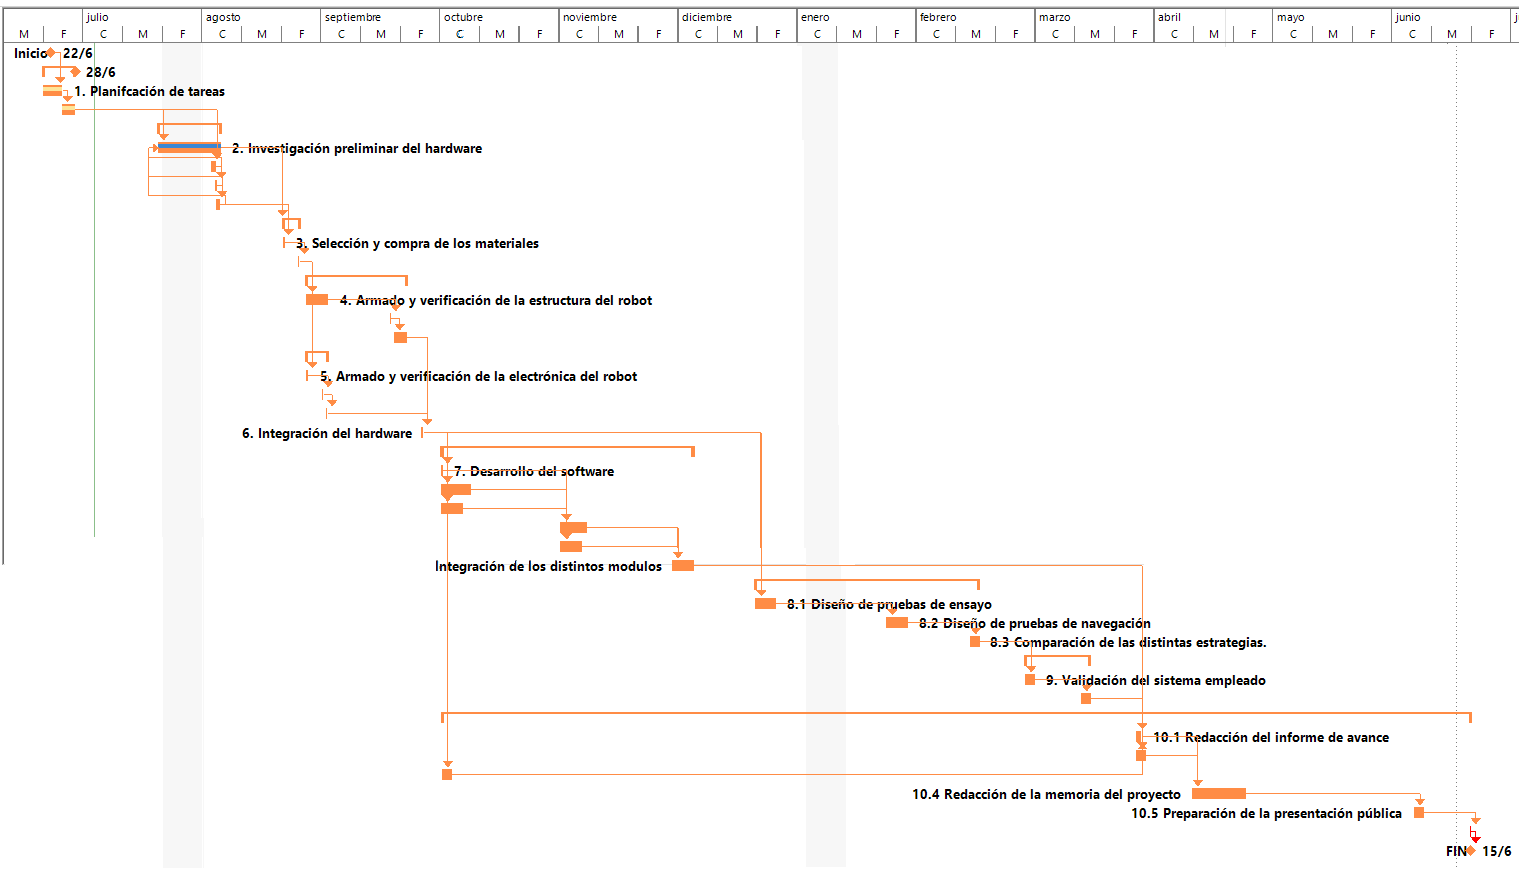
\includegraphics[width=1.6\textwidth]{./Figuras/gtant_fin.png}
\caption{Diagrama de \textit{Gantt}}
\label{fig:Gantt}
\end{figure}
\end{landscape}

\section{12. Presupuesto detallado del proyecto}
\label{sec:presupuesto}

\begin{consigna}{red}
Si el proyecto es complejo entonces separarlo en partes:
\begin{itemize}
	\item Un total global, indicando el subtotal acumulado por cada una de las áreas.
	\item El desglose detallado del subtotal de cada una de las áreas.
\end{itemize}

IMPORTANTE: No olvidarse de considerar los COSTOS INDIRECTOS.

\end{consigna}

\begin{table}[htpb]
\centering
\begin{tabularx}{\linewidth}{@{}|X|c|r|r|@{}}
\hline
\rowcolor[HTML]{C0C0C0} 
\multicolumn{4}{|c|}{\cellcolor[HTML]{C0C0C0}COSTOS DIRECTOS} \\ \hline
\rowcolor[HTML]{C0C0C0} 
Descripción &
  \multicolumn{1}{c|}{\cellcolor[HTML]{C0C0C0}Cantidad} &
  \multicolumn{1}{c|}{\cellcolor[HTML]{C0C0C0}Valor unitario} &
  \multicolumn{1}{c|}{\cellcolor[HTML]{C0C0C0}Valor total} \\ \hline
 &
  \multicolumn{1}{c|}{} &
  \multicolumn{1}{c|}{} &
  \multicolumn{1}{c|}{} \\ \hline
 &
  \multicolumn{1}{c|}{} &
  \multicolumn{1}{c|}{} &
  \multicolumn{1}{c|}{} \\ \hline
\multicolumn{1}{|l|}{} &
   &
   &
   \\ \hline
\multicolumn{1}{|l|}{} &
   &
   &
   \\ \hline
\multicolumn{3}{|c|}{SUBTOTAL} &
  \multicolumn{1}{c|}{} \\ \hline
\rowcolor[HTML]{C0C0C0} 
\multicolumn{4}{|c|}{\cellcolor[HTML]{C0C0C0}COSTOS INDIRECTOS} \\ \hline
\rowcolor[HTML]{C0C0C0} 
Descripción &
  \multicolumn{1}{c|}{\cellcolor[HTML]{C0C0C0}Cantidad} &
  \multicolumn{1}{c|}{\cellcolor[HTML]{C0C0C0}Valor unitario} &
  \multicolumn{1}{c|}{\cellcolor[HTML]{C0C0C0}Valor total} \\ \hline
\multicolumn{1}{|l|}{} &
   &
   &
   \\ \hline
\multicolumn{1}{|l|}{} &
   &
   &
   \\ \hline
\multicolumn{1}{|l|}{} &
   &
   &
   \\ \hline
\multicolumn{3}{|c|}{SUBTOTAL} &
  \multicolumn{1}{c|}{} \\ \hline
\rowcolor[HTML]{C0C0C0}
\multicolumn{3}{|c|}{TOTAL} &
   \\ \hline
\end{tabularx}%
\end{table}


\section{13. Gestión de riesgos}
\label{sec:riesgos}

\begin{consigna}{red}
a) Identificación de los riesgos (al menos cinco) y estimación de sus consecuencias:
 
Riesgo 1: detallar el riesgo (riesgo es algo que si ocurre altera los planes previstos de forma negativa)
\begin{itemize}
	\item Severidad (S): mientras más severo, más alto es el número (usar números del 1 al 10).\\
	Justificar el motivo por el cual se asigna determinado número de severidad (S).
	\item Probabilidad de ocurrencia (O): mientras más probable, más alto es el número (usar del 1 al 10).\\
	Justificar el motivo por el cual se asigna determinado número de (O). 
\end{itemize}   

Riesgo 2:
\begin{itemize}
	\item Severidad (S): 
	\item Ocurrencia (O):
\end{itemize}

Riesgo 3:
\begin{itemize}
	\item Severidad (S): 
	\item Ocurrencia (O):
\end{itemize}


b) Tabla de gestión de riesgos:      (El RPN se calcula como RPN=SxO)

\begin{table}[htpb]
\centering
\begin{tabularx}{\linewidth}{@{}|X|c|c|c|c|c|c|@{}}
\hline
\rowcolor[HTML]{C0C0C0} 
Riesgo & S & O & RPN & S* & O* & RPN* \\ \hline
       &   &   &     &    &    &      \\ \hline
       &   &   &     &    &    &      \\ \hline
       &   &   &     &    &    &      \\ \hline
       &   &   &     &    &    &      \\ \hline
       &   &   &     &    &    &      \\ \hline
\end{tabularx}%
\end{table}

Criterio adoptado: 
Se tomarán medidas de mitigación en los riesgos cuyos números de RPN sean mayores a...

Nota: los valores marcados con (*) en la tabla corresponden luego de haber aplicado la mitigación.

c) Plan de mitigación de los riesgos que originalmente excedían el RPN máximo establecido:
 
Riesgo 1: plan de mitigación (si por el RPN fuera necesario elaborar un plan de mitigación).
  Nueva asignación de S y O, con su respectiva justificación:
  - Severidad (S): mientras más severo, más alto es el número (usar números del 1 al 10).
          Justificar el motivo por el cual se asigna determinado número de severidad (S).
  - Probabilidad de ocurrencia (O): mientras más probable, más alto es el número (usar del 1 al 10).
          Justificar el motivo por el cual se asigna determinado número de (O).

Riesgo 2: plan de mitigación (si por el RPN fuera necesario elaborar un plan de mitigación).
 
Riesgo 3: plan de mitigación (si por el RPN fuera necesario elaborar un plan de mitigación).

\end{consigna}


\section{14. Gestión de la calidad}
\label{sec:calidad}

\begin{consigna}{red}
Para cada uno de los requerimientos del proyecto indique:
\begin{itemize} 
\item Req \#1: copiar acá el requerimiento.

\begin{itemize}
	\item Verificación para confirmar si se cumplió con lo requerido antes de mostrar el sistema al cliente. Detallar 
	\item Validación con el cliente para confirmar que está de acuerdo en que se cumplió con lo requerido. Detallar  
\end{itemize}

\end{itemize}

Tener en cuenta que en este contexto se pueden mencionar simulaciones, cálculos, revisión de hojas de datos, consulta con expertos, mediciones, etc.  Las acciones de verificación suelen considerar al entregable como ``caja blanca'', es decir se conoce en profundidad su funcionamiento interno.  En cambio, las acciones de validación suelen considerar al entregable como ``caja negra'', es decir, que no se conocen los detalles de su funcionamiento interno.

\end{consigna}

\section{15. Procesos de cierre}    
\label{sec:cierre}

\begin{consigna}{red}
Establecer las pautas de trabajo para realizar una reunión final de evaluación del proyecto, tal que contemple las siguientes actividades:

\begin{itemize}
	\item Pautas de trabajo que se seguirán para analizar si se respetó el Plan de Proyecto original:
	 - Indicar quién se ocupará de hacer esto y cuál será el procedimiento a aplicar. 
	\item Identificación de las técnicas y procedimientos útiles e inútiles que se emplearon, y los problemas que surgieron y cómo se solucionaron:
	 - Indicar quién se ocupará de hacer esto y cuál será el procedimiento para dejar registro.
	\item Indicar quién organizará el acto de agradecimiento a todos los interesados, y en especial al equipo de trabajo y colaboradores:
	  - Indicar esto y quién financiará los gastos correspondientes.
\end{itemize}

\end{consigna}


\end{document}
